\chapter{Materiais e Métodos\label{cap:metodologia}}

Antes de atacar o método em si foi necessário estudo de Algoritmos Genéticos e Linguagem C, escolhida pensando em CUDA.

%========================================================
\section{Autovalores de Hamiltonianos com Algoritmos Genéticos\label{sec:metodo}}
%========================================================

	Os métodos que estudei nessa dissertação estão contidos em uma série de artigos \cite{metodo2002, metodo2004, metodo2006, metodo2008, metodo2009, metodo2011}. O objetivo é encontrar, sequencialmente, do menor para o maior, os autovalores de uma matriz simétrica. Essa matriz é o Hamiltoniano presente na formulação matricial da equação de Schrödinger independente do tempo\footnote{Ela é importante para a física moderna pois está associada à quantização da energia na Mecânica Quântica. No apêndice \ref{apdc:eqSchr} há uma breve exposição de como essa equação diferencial parcial pode ser escrita como um problema de autovalores e autovetores.}. A estratégia é transformar o problema do autovalor em um problema de otimização, buscando um escalar $a_i$ e um vetor $X_i$ de modo que a equaçaõ $HX_i = a_iX_i$ seja satisfeita.
	
	Os algoritmos apresentados em \cite{metodo2004} e \cite{metodo2011} são mais simples. Por exemplo, em \cite{metodo2002} o Hamiltoniano é alterado por rotações de Jacobi e, só então, o \emph{fitness} é calculado. Nos artigos \cite{metodo2006}, \cite{metodo2008} e \cite{metodo2009} o espaço vetorial é dividido em duas partes de dimensões diferentes, levando a um Hamiltoniano que contém alguns autovalores de interesse\footnote{\emph{Partitioned matrix eigenvalue problem.}}. Isso não ocorre com os GAs das publicações de 2004 e 2011. Nelas o Hamiltoniano original é sempre mantido.
	
	Pode-se dizer que \cite{metodo2011} é a continuação de \cite{metodo2004}. A representação cromossomial e os operadores de seleção, \emph{crossover} e mutação são os mesmos. No entanto, ele adiciona dois operadores genéticos. O primeiro é complementar à mutação, e atua para criar mais diversidade na população. O segundo acentua a pressão seletiva via Elitismo. Não há justificativa para os novos operadores. Acredito que o intuito tenha sido melhorar a qualidade dos resultados, mas, infelizmente, não há comparação com os obtidos em 2004. E, de fato, isso seria impossível, pois em 2011 há uma mudança drástica: a função de avaliação foi alterada. Além disso, \cite{metodo2011} paraleliza o GA e compara os desempenhos.
	
	Assim, optei por seguir estritamente o processo e os operadores discutidos em \cite{metodo2004}, mas utilizar, também, o \emph{fitness} do \cite{metodo2011}. Ao manter o mesmo GA, foi possível comparar com segurança os resultados das duas funções de avaliação.

%========================================================	
\section{Descrição do Algoritmo Genético}
%========================================================	

	Há casos em que não há solução exata para a equação de Schrödinger independente do tempo. Quando isso acontece, é preciso introduzir uma base ortonormal finita {$\phi$} e expandir o estado estacionário $\psi$ em termos dos vetores geradores dessa base
	
	\begin{equation}
		\psi = \sum_k c_k \phi_k.
	\end{equation}
	
	Isso leva ao problema de autovalores
	
	\begin{equation}\label{eq:HCEC}
		HC = EC,
	\end{equation}
	onde $H$ é uma matriz real e simétrica, construída na base ${\phi}$, que representa o operador Hamiltoniano. A diagonalização de $H$ encontra os autovalores $E_n$ correspondentes às energias possíveis do sistema quântico. Com isso, é possível obter os autovetores (autoestados) $C_n$ associados.
	
	No artigo \cite{metodo2004} é apresentada uma maneira de reduzir o problema de autovalores a um problema de busca. Dados todos os vetores $C$ existentes na base $\phi$, conjunto chamado de \textbf{Espaço de Busca}, o objetivo é encontrar os autovetores $C_n$ que satisfaçam a equação \ref{eq:HCEC}. O conjunto de todos os autovetores $C_n$ é o \textbf{Espaço de Soluções}. O mecanismo de busca é um algoritmo genético (GA).
	
	Conforme visto no capítulo \ref{cap:ga}, o elo entre o GA e o problema a ser resolvido está na Representação Cromossomial e na Função de Avaliação. O cromossomo deve codificar a solução desejada na forma de um \emph{string}, seja de caracteres, símbolos, números inteiros ou reais. O \emph{fitness} deve ser capaz de definir, objetivamente, a qualidade de todos os indivíduos da população, de modo que seja possível comparar cada um com as soluções desejadas. Quanto mais próximo um cromossomo está da solução, mais alto deve ser seu \emph{fitness}.

%-------------------------------------------------------		
	\subsection{Representação Cromossomial}
%-------------------------------------------------------	
	
	Como solução pretendida é um autovetor, o cromossomo codifica um vetor. Cada indivíduo $i$ da população é um vetor $\psi_i$ candidato à autovetor na forma
	
	\begin{equation}
		\psi_i = \sum_{p=1}^m c_{pi}\phi_p, \mbox{   } i = 1,2, \cdots, n
	\end{equation}
	
	Na equação acima, $i$ varia de 1 até o número máximo de indivíduos na população do GA, mantida fixa ao longo de toda a execução. O índice $p$ é tomado de 1 até a $m$, que é ordem da matriz $H$ (ou a dimensão do espaço vetorial).
	
	O cromossomo é definido como uma cadeia de números reais, cujos valores são os coeficientes $c_{pi}$. O \emph{string} $S_i$, codificação para o membro $\psi_i$, é dado por
	
	\begin{equation}
		S_i \equiv  (c_{1i}, c_{2i}, \cdots, c_{pi}, \cdots, c_{mi}) = C^{\dagger}_i,
	\end{equation}
	enquanto que para outro membro $\psi_k$ da população, o \emph{string} $S_k$ é
	
	\begin{equation}
		S_k \equiv  (c_{1k}, c_{2k}, \cdots, c_{pk}, \cdots, c_{mk}) = C^{\dagger}_k.
	\end{equation}
	
%-------------------------------------------------------
	\subsection{População}
%-------------------------------------------------------

	A população inicial é gerada aleatoriamente. Seu tamanho (número de indivíduos) é sempre mantido fixo a cada nova geração.
	
%-------------------------------------------------------
	\subsection{Funções de Avaliação (\emph{fitness})}
%-------------------------------------------------------	

	O \emph{fitness} proposto em \cite{metodo2004} é obtido em três passos:
	
	\begin{enumerate}
		\item \label{item:passo1} Cálculo do quociente de Rayleigh $\rho_i$ associado ao $i-$ésimo indivíduo $C_i$;
		\item \label{item:passo2} Cálculo do gradiente de $\rho_i$;
		\item \label{item:passo3} Cálculo da função de avaliação.
	\end{enumerate}
	
	Retomando o capítulo \ref{cap:algebra}, o quociente de Rayleigh é dado por
	
	\begin{equation}
		\rho_i = \frac{C_i^\dagger H C_i}{C_i^\dagger C_i},
	\end{equation}
	e seu gradiente por
	
	\begin{equation}\label{eq:grad_rho_metodo}
		\nabla \rho_i = \frac{2[H - \rho_i]C_i}{C_i^\dagger C_i}.
	\end{equation}
		
	O \emph{fitness} é então definido como \footnote{
		No artigo \cite{metodo2004} a equação originalmente apresentada é $f_i = e^{-\lambda (\nabla \rho_i)^{\nabla \rho_i}}$. Acredito que tenha sido um erro de digitação por dois motivos. O primeiro é que tal definição não leva, necessariamente, ao comportamento esperado: $f_i \rightarrow 1$ quando $\nabla \rho_i \rightarrow 0$. Em segundo lugar, nos artigos \cite{metodo2006},  \cite{metodo2008} e \cite{metodo2009}, que seguem o mesmo método, a função de avaliação é definida como $f_i = e^{-\lambda (\nabla \rho_i)^{\dagger} (\nabla \rho_i)}$. Portanto, segui com a definição de $f_i$ da equação \ref{eq:fitness_extenso}.}
	
	\begin{equation}\label{eq:fitness_extenso}
		f_i = e^{-\lambda (\nabla \rho_i)^\dagger (\nabla \rho_i)}.
	\end{equation}
	
	Lembrando que o módulo de um vetor $V$ é dado por $|V| = \sqrt{V^{\dagger} V}$, a equação \ref{eq:fitness_extenso} fica
	
	\begin{equation}\label{eq:fitness_grad}
		f_i(\nabla \rho_i) = e^{-\lambda |\nabla \rho_i|^2}.
	\end{equation}
			 
	A função de avaliação $f_i$ está limitada entre zero e um, $f_i$ = (0,1]. Se $|\nabla \rho|^2 \gg 0$, $f_i \rightarrow 0$, indicando que $C_i$ possui baixa qualidade, está longe da solução. Por outro lado, se $\nabla \rho_i \rightarrow 0 $, $f_i \rightarrow 1$, e $C_i$ é uma boa aproximação para um autovetor. O parâmetro $\lambda$ é escolhido para não haver \emph{over flow} ou \emph{under flow} da função exponencial.
	
	De acordo com os autores, a equação \ref{eq:fitness_grad} leva ao autovalor mínimo. Se algum $C_i$, em algum momento, é o autovetor fundamental $C_0$, o $\nabla \rho$ é nulo. Eles afirmam que ``\textit{Claramente, $f_i \rightarrow 1$ quando $\nabla \rho_i \rightarrow 0$, sinalizando que a evolução atingiu o verdadeiro autovetor fundamental de $H$ em $C_i$}''\footnote{Tradução livre de ``\textit{Clearly, $f_i \rightarrow 1$, as $\nabla \rho_i \rightarrow 0$, signalling that the evolution has hit the true ground state eigenvector of $H$ in the vector $C_i$}''.}. 
	
	Uma vez que $C_0$ foi encontrado, o próximo passo é obter o autovalor $E_0$ associado. Na verdade ele já foi calculado, e é simplesmente o valor do quociente de Rayleigh para $C_i$:
	
	\begin{equation}
		\rho_0 = \frac{C_i^{\dagger} H C_i}{C_i^{\dagger} C_i} = E_0.
	\end{equation}
	
	Quando o algoritmo chega nesse estágio tem-se o par $(C_0,E_0)$.
	
	Como já dito anteriormente, a função de avaliação foi alterada em \cite{metodo2011}, e é dada por 
	
	\begin{equation}\label{eq:fitness_EL_metodo}
		f_i(\rho_i) = e^{-\lambda(\rho_i - E_L)^2},
	\end{equation}
	onde $E_L$ é um limite inferior para o autovalor mínimo procurado.
	
	Ela compartilha algumas propriedades com a equação \ref{eq:fitness_grad}. Está limitada no conjunto $f_i(\rho) = (0,1]$ e, quanto maior seu valor, melhor a qualidade do indivíduo. O parâmetro $\lambda$ tem exatamente a mesma função. A busca utilizando $f_i(\rho)$ também termina quando $f_i \rightarrow 1$. ``\emph{Se $\rho_i \rightarrow E_L$ durante a busca, $f_i \rightarrow 1$ and $C_i$ se aproxima do autovetor fundamental de $H$}''. Novamente, como já temos $C_0$, o autovalor $E_0$ é simplesmente o $\rho_i$ já calculado.	O cálculo de $f_i(\rho)$ executa os passos \ref{item:passo1} e \ref{item:passo3} de $f_i(\nabla\rho)$.
				
		A não ser por acidente, a condição $f_i \rightarrow 1$ não é satisfeita logo na primeira população. É necessário evoluir os indivíduos por meio dos operadores genéticos de seleção, reprodução e mutação. Eles serão apresentados nas seções seguintes.

%-------------------------------------------------------
\subsection{Seleção}
%-------------------------------------------------------	

			O operador de seleção utilizado tanto em \cite{metodo2004} quanto em \cite{metodo2011} é o da Roleta, com fatias proporcionais aos valores do \emph{fitness} \cite{Linden2008}. Se a população possui $q$ indivíduos, a roleta é ``girada'' $q$ vezes, de modo a criar a nova população com os $q$ cromossomos selecionados.
			
			Entretanto, utilizei a seleção por Torneio pelos motivos apresentados na seção \ref{sec:torneio}. Mantive o tamanho da população fixa.
									
%-------------------------------------------------------
\subsection{Reprodução}
%-------------------------------------------------------

	A operação de reprodução ($crossover$) é aplicada na nova população após a Seleção. Há diferença entre os operadores de reprodução de \cite{metodo2004} e \cite{metodo2011}. Apresentarei ambos e, ao final, justificarei porque escolhi como base o segundo.

%----------------------------------------------------	
\subsubsection{\emph{Crossover} em \cite{metodo2004}}
%----------------------------------------------------	
	
	Suponha que tenham sido escolhidos, aleatoriamente, um par de cromossomos ($S_k$, $S_l$) dentre todos os $N$ indivíduos da população:
	
	\begin{equation}
		\begin{array}{l}
			S_k = (c_{k1}, c_{k2}, \cdots, c_{kn})	\\
			S_l = (c_{l1}, c_{l2}, \cdots, c_{ln})	
		\end{array}
	\end{equation}

	Em seguida, um inteiro $p$ é obtido, também aleatoriamente, entre 1 e $n - 1$ [p = [$1$, $n$)]. Lembre-se que $n$ é a ordem da matriz $H$ e, portanto, a quantidade de coeficientes no \emph{string} $S_i$. A função de $p$ é determinar em qual posição (\emph{locus}) do cromossomo acontecerá a alteração.
	
	O operador cria o novo par ($S^{'}_k$, $S^{'}_l$):
	
	\begin{equation}
		\begin{array}{l}
			S^{'}_k = (c_{k1}, c_{k2}, \cdots, c^{'}_{kp} c_{k,p+1}, \cdots, c_{kn})	\\
			S^{'}_l = (c_{l1}, c_{l2}, \cdots,  c^{'}_{lp} c_{l,p+1}, \cdots, c_{ln}),	\\
			
		\end{array}
	\end{equation}
	onde
	
	\begin{equation}
		\begin{array}{l}
			c^{'}_{kp} = f c_{kp} + (1 - f) c_{lp}     \\
			c^{'}_{lp} = (1 - f) c_{kp} + f c_{lp}.
		\end{array}
	\end{equation}
	
	O parâmetro $f$ faz o papel da mistura que cria nova informação. Ele é gerado aleatoriamente com valores entre zero e um. Nesse caso os valores limite não estão inclusos [f = (0,1)]. Dessa maneira há garantia de mistura.
	
	Esse operador só age em uma certa fração da população, dada por uma probabilidade $p_c$ que, em geral, é grande (70$-$75\%). O restante da população não é alterado.

%-----------------
\textbf{Exemplo}.
%-----------------

Na figura \ref{fig:cross2004_tabelaAntes} há dois cromossomos de tamanho $n = 6$. A posição onde ocorrerá a alteração dos valores foi obtida aleatoriamente entre $p = [1,6)$, e, para esse caso, vale $p = 4$. O valor de $S_k$ na posição $p = 4$ é $c_{k4} = 0,80$, e para $S_l$ é $c_{l4} = 0,39$. Para $p + 1$ os valores são $c_{k5} = 0,15$ e $c_{l5} = 0,89$.

\begin{figure}[htbp]
	\centering
		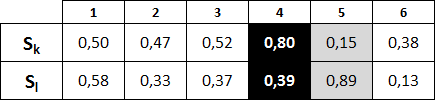
\includegraphics[width=0.70\textwidth]{figs/materiais_metodo/autovalores_com_ga/cross2004_tabelaAntes.png}
	\caption{Exemplo do \emph{crossover} de \cite{metodo2004}. Indivíduos antes da reprodução.}
	\label{fig:cross2004_tabelaAntes}
\end{figure}

O parâmetro $f$ teve seu valor determinado aleatoriamente como $f = 0,62$. Os valores de $c^{'}_{k4}$ e $c^{'}_{l4}$ ficam:

\begin{equation}\label{eq:ck4}
	\begin{array}{lccl}
		c^{'}_{kp} = & f c_{kp} & + & (1 - f) c_{lp} 						\\
		c^{'}_{k4} = & 0,62 c_{k4} & + & (1 - 0,62) c_{l4} 			\\
		c^{'}_{k4} = & 0,62 * 0,80 & + & 0,38 * 0,39 						\\		
		c^{'}_{k4} = & 0,496 & + & 0,1482	\\		
		c^{'}_{k4} = & 0,6442 &  & 
	\end{array}
\end{equation}

\begin{equation}\label{eq:cl4}
	\begin{array}{lccl}
		c^{'}_{lp} = & (1-f) c_{kp} & + & f c_{lp} 						\\
		c^{'}_{l4} = & (1-0,62) c_{k4} & + & 0,62 c_{l4} 						\\
		c^{'}_{l4} = & 0,38 * 0,80 & + & 0,62 * 0,39 						\\
		c^{'}_{l4} = & 0,304 & + & 0,2418 						\\
		c^{'}_{l4} = & 0,5458 &  & 
	\end{array}
\end{equation}

Finalmente, os valores para a posição $p = 4$ nos novos indivíduos $S^{'}_k$ e $S^{'}_l$ são

\begin{equation}\label{eq:cross2004_novo_valor_sk}
	\begin{array}{ll}
	\mbox{Novo valor na posição 4 de  } S^{'}_k & = c^{'}_{kp} c_{k,p+1} \\
								& = c^{'}_{k4} c_{k5} \\
								& = 0,6442 * 0,15	\\
								& = 0,09663	\\
								& \approx 0,1
	\end{array}
\end{equation}

\begin{equation}\label{eq:cross2004_novo_valor_sl}
	\begin{array}{ll}
	\mbox{Novo valor na posição 4 de  } S^{'}_l & = c^{'}_{lp} c_{l,p+1} \\
								& = c^{'}_{l4} c_{l5} \\
								& = 0,5458 * 0,89	\\
								& = 0,485762 \\
								& \approx  0,49
	\end{array}
\end{equation}


Na figura \ref{fig:cross2004_tabelaDepois} há os dois novos indivíduos.

\begin{figure}[htbp]
	\centering
		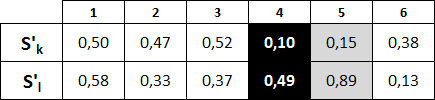
\includegraphics[width=0.70\textwidth]{figs/materiais_metodo/autovalores_com_ga/cross2004_tabelaDepois.png}
	\caption{Exemplo do \emph{crossover} de \cite{metodo2004}. Indivíduos depois da reprodução.}
	\label{fig:cross2004_tabelaDepois}
\end{figure}

%----------------------------------------------------
\subsubsection{\emph{Crossover} em \cite{metodo2011}}	
%----------------------------------------------------

	A representação cromossomial usada em \cite{metodo2011} é a mesma de \cite{metodo2004}, portanto, o par ($S_k$, $S_l$) é igual, assim como a probabilidade $p_c$:
	
	\begin{equation}
		\begin{array}{l}
		S_k = (c_{k1}, c_{k2}, \cdots, c_{kn})	\\
		S_l = (c_{l1}, c_{l2}, \cdots, c_{ln})	
		\end{array}
	\end{equation}
	
	Diferentemente de \cite{metodo2004}, utiliza-se o \emph{crossover} de dois pontos. Aleatoriamente escolhe-se dois inteiros, $o$ e $p$, cuja função é determinar a região do cromossomo que sofrerá miscigenação. O valor em $o$ indica o primeiro gene, e $p$ o último. Portanto, todos os genes entre os dois, incluindo eles próprios, sofrerão a ação do \emph{crossover} ($o <= c_i <= p$, $p \geq o$). Os novos indivíduos são ($S^{'}_k$, $^{'}S_l$)
	
	\begin{equation}
		\begin{array}{l}
			S^{'}_k = (c_{k1}, c_{k2}, \cdots, c^{'}_{ko}, \cdots , c^{'}_{kp}, c_{k,p+1}, \cdots, c_{kn})	\\
			S^{'}_l = (c_{l1}, c_{l2}, \cdots, c^{'}_{lo}, \cdots , c^{'}_{lp}, c_{l,p+1}, \cdots, c_{ln}).	
		\end{array}
	\end{equation}
	
	Para todos genes selecionados, a transformação ocorre da seguinte maneira ($i = o, o + 1, \cdots, p$):
	
	\begin{equation}
		\begin{array}{l}
			c^{'}_{ki} = f_c c_{ki} + (1 - f_c) c_{li}     \\
			c^{'}_{li} = (1 - f_c) c_{ki} + f_c c_{li}
		\end{array}
	\end{equation}
	onde $f_c$ é dado por
	
	\begin{equation}
		f_c = 0,75 + 0,25r,
	\end{equation}
	sendo $r$ um número aleatório ($0 \leq r \leq 1$). Assim como o parâmetro $f$ de \cite{metodo2004}, $f_c$ faz o papel da mistura que cria nova informação.
	
	\textbf{Exemplo}.
	
	
	Usei os mesmos indivíduos da figura \ref{fig:cross2004_tabelaAntes}. Os parâmetros $o$ e $p$ foram escolhidos no intervalo [1,6] e têm valores $o = 2$ e $p = 4$. Portanto, no \emph{string} $S_k$ os elementos que sofrerão alteração são $c_{k2} = 0,47$, $c_{k3} = 0,52$ e $c_{k4} = 0,80$. Eles se misturarão com os elementos $c_{l2} = 0,33$, $c_{l3} = 0,37$ e $c_{l4} = 0,39$ de $S_l$. Aleatoriamente obtive $r = 0,2$, que leva a $f_c = 0,80$.
	
	\begin{figure}[htbp]
	\centering
		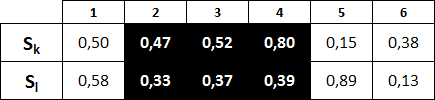
\includegraphics[width=0.70\textwidth]{figs/materiais_metodo/autovalores_com_ga/cross2011_tabelaAntes.png}
	\caption{Exemplo do \emph{crossover} de \cite{metodo2011}. Indivíduos antes da reprodução.}
	\label{fig:cross2011_tabelaAntes}
\end{figure}
	
	Os elementos $c^{'}_{ki}$ são:
	
	\begin{equation}
		\begin{array}{llcl}
			c^{'}_{k2}	& = f_c c_{k2} 		& + & (1- f_c) c_{l2} \\
									& = 0,80 * 0,47		& + &	(1 - 0,80) * 0,33 \\
									& = 0,376					& + & 0,2 * 0,33	\\
									& = 0,376					& + & 0,066	\\
									& = 0,442 \\
									& \approx 0,44
		\end{array}
	\end{equation}
	
	
	\begin{equation}
		\begin{array}{llcl}
			c^{'}_{k3}	& = f_c c_{k3} 		& + & (1- f_c) c_{l3} \\
									& = 0,80 * 0,52		& + &	(1 - 0,80) * 0,37 \\
									& = 0,416					& + & 0,2 * 0,37	\\
									& = 0,416					& + & 0,074	\\
									& = 0,49
		\end{array}
	\end{equation}
	
	
	\begin{equation}
		\begin{array}{llcl}
			c^{'}_{k4}	& = f_c c_{k4} 		& + & (1- f_c) c_{l4} \\
									& = 0,80 * 0,80		& + &	(1 - 0,80) * 0,39 \\
									& = 0,64					& + & 0,2 * 0,39	\\
									& = 0,64					& + & 0,078	\\
									& = 0,718 \\
									& \approx 0,72
		\end{array}
	\end{equation}
	
	
	Os elementos $c^{'}_{li}$ são:
	
	\begin{equation}
		\begin{array}{llcl}
			c^{'}_{l2}	& = (1 - f_c) c_{k2} 		& + & f_c c_{l2} \\
									& = (1 - 0,80) * 0,47		& + &	0,80 * 0,33 \\
									& = 0,2 * 0,47					& + & 0,264	\\
									& = 0,094					& + & 0,264	\\
									& = 0,358 \\
									& \approx 0,36
		\end{array}
	\end{equation}
	
	\begin{equation}
		\begin{array}{llcl}
			c^{'}_{l3}	& = (1 - f_c) c_{k3} 		& + & f_c c_{l3} \\
									& = (1 - 0,80) * 0,52		& + &	0,80 * 0,37 \\
									& = 0,2 * 0,52					& + & 0,296	\\
									& = 0,104								& + & 0,296	\\
									& = 0,40									
		\end{array}
	\end{equation}
	
	
	\begin{equation}
		\begin{array}{llcl}
			c^{'}_{l4}	& = (1 - f_c) c_{k4} 		& + & f_c c_{l4} \\
									& = (1 - 0,80) * 0,80		& + &	0,80 * 0,39 \\
									& = 0,2 * 0,80					& + & 0,312	\\
									& = 0,16								& + & 0,312	\\
									& = 0,472 \\
									& \approx 0,47
		\end{array}
	\end{equation}
	
	Os novos indivíduos estão na figura \ref{fig:cross2011_tabelaDepois}.
		
	\begin{figure}[htbp]
	\centering
		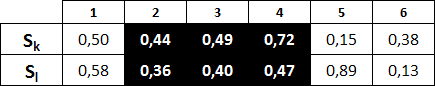
\includegraphics[width=0.70\textwidth]{figs/materiais_metodo/autovalores_com_ga/cross2011_tabelaDepois.png}
	\caption{Exemplo do \emph{crossover} de \cite{metodo2011}. Indivíduos depois da reprodução.}
	\label{fig:cross2011_tabelaDepois}
\end{figure}
	
	
%----------------------------------------------------
\subsubsection{\emph{Crossover} utilizado}	
%----------------------------------------------------

	A quantidade de nova informação não é escalável com o tamanho do cromossomo no \emph{crossover} de \cite{metodo2004}. Ele altera apenas uma posição (locus) de cada indivíduo, independentemente do tamanho do cromossomo. Por exemplo, se a ordem do Hamiltoniano for $n = 100$, o \emph{string} terá 100 elementos, mas apenas um sofrerá alteração. O mesmo aconteceria para $n = 1.000$, 10.000 e assim por diante.
	
	Ainda sobre o artigo de 2004, é impossível haver troca de informação na última posição. O parâmetro $p$, obtido aleatoriamente, dá a posição que ocorrerá o \emph{crossover}. Porém, parte do cálculo envolve os elementos $c_{k,p+1}$ e $c_{l,p+1}$. Note o índice $p+1$. Como a posição máxima é $n$, o maior índice possível para estes elementos é $p + 1 = n$, impondo o limite $p \leq n - 1$. Nos exemplos apresentados, $n = 6$, $p \leq 5$ e, portanto, a posição $6$ nunca será escolhida.
	
	Isso pode dificultar a busca. Suponhe que uma solução precise do valor 23 no último coeficiente do cromossomo ($c_n = 0,23$). Se nenhum indivíduo da população inicial já tiver nascido com ele, esse valor nunca aparecerá por meio do \emph{crossover}. Resta como esperança a Mutação, porém, por definição, ela tem baixa probabilidade \cite{Linden2008}. Também não há garantia de que, após muitas gerações com sucessivas operações de \emph{crossover}, mutação e seleção, haverá um indivíduo na população que, além de ter 0,23 na última posição, possua os outros $(n-1)$ primeiros elementos necessários.
		
		O \emph{crossover} de \cite{metodo2004} é um caso especial do \emph{crossover} de \cite{metodo2011}. O operador de reprodução de \cite{metodo2011} é o clássico \emph{crossover} de dois pontos \cite{Linden2008}. Nele, $p \geq o$, e, se $o = p$, há mistura em apenas uma posição do \emph{string}, exatamente o que acontece em \cite{metodo2004}. Como $1 \leq o \leq n$ e $1 \leq p \leq n$, o último gene também está sujeito à operação, e o problema citado no parágrafo anterior não existe.
		
	Pelo que expus acima, escolhi utilizar o \emph{crossover} de \cite{metodo2011}, mas com uma pequena modificação. No cálculo dos novos coeficientes $c^{'}_{i}$, invés do parâmetro $f_c$, usei o $f$ conforme definido em \cite{metodo2004}. O $f$ pode variar entre $0$ e $1$, enquanto o $f_c$, além de necessitar do parâmetro adicional $r$, é limitado apenas entre $0,75$ e $1$. Assim, acredito que $f$ seja mais abrangente como parâmetro de mistura e criação de nova informação.
	
	A seguir apresento sinteticamente a estrutura do \emph{crossover} utilizado. Um par de indivíduos $(S_k, S_l)$
	
	\begin{equation}
		\begin{array}{l}
			S_k = (c_{k1}, c_{k2}, \cdots, c_{kn})	\\
			S_l = (c_{l1}, c_{l2}, \cdots, c_{ln})	
		\end{array}
	\end{equation}
	é obtido aleatoriamente da população. Com probabilidade $p_c$, a operação de \emph{crossover} acontece. Dois pontos de corte $o$ e $p$ são obtidos, também aleatoriamente, gerando os novos \emph{strings} $S^{'}_k$ e $S^{'}_l$ na forma
		
	\begin{equation}
		\begin{array}{l}
			S^{'}_k = (c_{k1}, c_{k2}, \cdots, c^{'}_{ko}, \cdots , c^{'}_{kp}, c_{k,p+1}, \cdots, c_{kn})	\\
			S^{'}_l = (c_{l1}, c_{l2}, \cdots, c^{'}_{lo}, \cdots , c^{'}_{lp}, c_{l,p+1}, \cdots, c_{ln}),
		\end{array}
	\end{equation}
	onde
	
	\begin{equation}
		\begin{array}{l}
			c^{'}_{ki} = f c_{ki} + (1 - f) c_{li}     \\
			c^{'}_{li} = (1 - f) c_{ki} + f c_{li}
		\end{array}
	\end{equation}
	e
	
	\begin{equation}
	0 \leq f \leq 1 \mbox{       (obtido aleatoriamente)}
	\end{equation}
	
-----------------

	Apresentar e definir a matriz de Coope-Sabo (citar artigo original de 77), utilizada no pelos indianos no artigo de 2006.


\section{CUDA}

Metodologia: revisão bibliográfica e aplicação no ONEMAX.

Material do ERAD.

\section{Framework/Programa Serial}

	Optou-se por desenvolver do zero todo o programa. Motivo: controle sobre todas as características do método.

	Linguagem C: linguagem nativa para CUDA.

	Totalmente parametrizado. 

	Com foi será possível:

	\begin{enumerate}
		\item Estudo do método 
		\item Estudo de algoritmos genéticos
		\item Novas aplicações como máximo de função
		\begin{enumerate}
			\item Mudança no fitness 
			\item Mudança nos critérios de parada
		\end{enumerate}	
	\end{enumerate}


	Descrição dos parâmetros.

	Descrição de cada função, incluindo \textit{print screen} das partes de código mais fundamentais:

	\begin{enumerate}
		\item Estruturas de dados
		\item Geração de números pseudoaleatórios
		\item Geração das Matrizes de Coope
		\item Geração da População Inicial
		\item Fitness: as várias equações
		\item Fitness: cálculo de $\rho_i$
		\item Fitness: cálculo de $\nabla\rho_i$
		\item Seleção
		\item Crossover
		\item Mutação
		\item Álgebra Linear: multiplicação de matrizes
		\item Álgebra Linear: multiplicação de matriz por escalar
		\item Álgebra Linear: subtração de matrizes
	\end{enumerate}

	Qualidade dos números pseudo-aleatórios (base do GA)
	
	

	\begin{enumerate}
			\item Mostrar que a distribuição dos números segue o esperado para números aleatórios
			\item Quanto maior a quantidade de pontos, melhor a distribuição
			\item Gráfico: histograma de frequência.
	\end{enumerate}

	Exemplo de execução no Windows.

	Reprodutibilidade.
	
	Exemplo de reprodutibilidade.

	Código disponível em

	\texttt{https://github.com/prietoab/msc\_code}